\subsection{Compute the crime rate per household. Generate a table of descriptive statistics of all the
variables that have been introduced so far. Comment on the descriptive statistics.}
% latex table generated in R 4.2.1 by xtable 1.8-4 package
% Wed Dec  6 21:45:13 2023
\begin{table}[ht]
\centering
\begin{tabular}{llllllr}
  \hline
var & median & mean & min & max & sd & NAs \\ 
  \hline
agro\_emp & 18.6 & 25.1 & 0.1 & 86.3 & 22.3 &  30 \\ 
  bribery & 11.7 & 17.0 & 0.0 & 67.1 & 14.7 &  87 \\ 
  gfce & 16.5 & 17.7 & 5.1 & 62.9 & 8.4 &  36 \\ 
  literacy & 93.0 & 83.6 & 24.2 & 100.0 & 19.3 &  61 \\ 
  log\_gdp & 9.4 & 9.3 & 6.6 & 11.6 & 1.2 &  22 \\ 
  pop\_total & 6.2e+06 & 3.4e+07 & 1.1e+04 & 1.4e+09 & 1.4e+08 &   2 \\ 
  self\_emp & 35.0 & 40.9 & 0.4 & 94.8 & 27.0 &  30 \\ 
  stocks & 6.4 & 28.8 & 0.0 & 538.7 & 66.8 & 131 \\ 
  sample\_size & 715.1 & 3.6e+03 & 120.1 & 1.4e+05 & 1.3e+04 &   2 \\ 
   \hline
\end{tabular}
\caption{Descriptive statistics} 
\label{desc}
\end{table}


Table \ref{desc2} shows the descriptive statistics of the table made of
900 hundred municipalities. First, the data is remarkably clean as their is no
NA values in it. For a clearer view I displayed the relative standard deviation (rsd)
defined as the standard deviation divided by the mean. I still have to comment on
this table but I don't know what to say.
\subsection{Estimate the model in equation (7) using OLS.}

% Table created by stargazer v.5.2.3 by Marek Hlavac, Social Policy Institute. E-mail: marek.hlavac at gmail.com
% Date and time: Ven, déc 08, 2023 - 16:57:32
% Requires LaTeX packages: dcolumn 
\begin{table}[!htbp] \centering 
  \caption{Ordinary Least Square Estimation - Exercise 3} 
  \label{results2} 
\begin{tabular}{@{\extracolsep{5pt}}lD{.}{.}{-3} } 
\\[-1.8ex]\hline 
\hline \\[-1.8ex] 
 & \multicolumn{1}{c}{\textit{Dependent variable:}} \\ 
\cline{2-2} 
\\[-1.8ex] & \multicolumn{1}{c}{crime\_rate} \\ 
\hline \\[-1.8ex] 
 business\_crea & 0.018^{***} \\ 
  & (0.005) \\ 
  & \\ 
 log(pop) & 0.001^{***} \\ 
  & (0.0002) \\ 
  & \\ 
 income & 0.00001 \\ 
  & (0.0001) \\ 
  & \\ 
 com\_typeC & -0.003^{***} \\ 
  & (0.0003) \\ 
  & \\ 
 com\_typeI & -0.002^{***} \\ 
  & (0.001) \\ 
  & \\ 
 Constant & 0.001 \\ 
  & (0.002) \\ 
  & \\ 
\hline \\[-1.8ex] 
Observations & \multicolumn{1}{c}{899} \\ 
R$^{2}$ & \multicolumn{1}{c}{0.150} \\ 
Adjusted R$^{2}$ & \multicolumn{1}{c}{0.145} \\ 
Residual Std. Error & \multicolumn{1}{c}{0.004 (df = 893)} \\ 
F Statistic & \multicolumn{1}{c}{31.568$^{***}$ (df = 5; 893)} \\ 
\hline 
\hline \\[-1.8ex] 
\textit{Note:}  & \multicolumn{1}{r}{$^{*}$p$<$0.1; $^{**}$p$<$0.05; $^{***}$p$<$0.01} \\ 
\end{tabular} 
\end{table} 

The coefficient of interest that results from the OLS (see Table \ref{results2}) is significantly different from zero at the 1\% level, and positive.
This is very unexpected as it would mean that the better the shape of the economy, the higher the crime rate. This result
could derive from endogeneity issues as an ommited variable bias for instance.
The fact that the coefficient of interest is positive while we expect it to be negative
means that the endogeneity issues are more than just measurment error as this kind of
problem leads underestimations (in absolute value) of the true coefficient.

\subsection{After estimating the model in equation (7), you wonder whether enodegeneity is a problem.
Why could the variable of interest, the business creation growth rate, be endogenous?}
As mentioned in the previous question, the fact that the estimation for the coefficient of interest is positive
leads to thinking about an ommited variable bias. For instance, both the shape of the economy and the crime rate could
be related to the level of inequality in the area. To inspect this hypothesis, we used the
iqr\_income variable which is defined as the difference between the first and third quartiles of income.
This is a proxy for the local level of inequality. Figure \ref{ineq} displays the crime rate and the business creation growth rate
against the iqr\_income variable. Even though the result is not cristal clear, we still find some positive correlation for both
the dependant and the explanatory variable. This is a source of enodegeneity. The coefficient of correlation with iqr\_income are respectively 0.23 and 0.082 for the business creation rate and the crime rate. 
\begin{figure}[htbp]
    \begin{minipage}{0.5\textwidth}
      \centering
      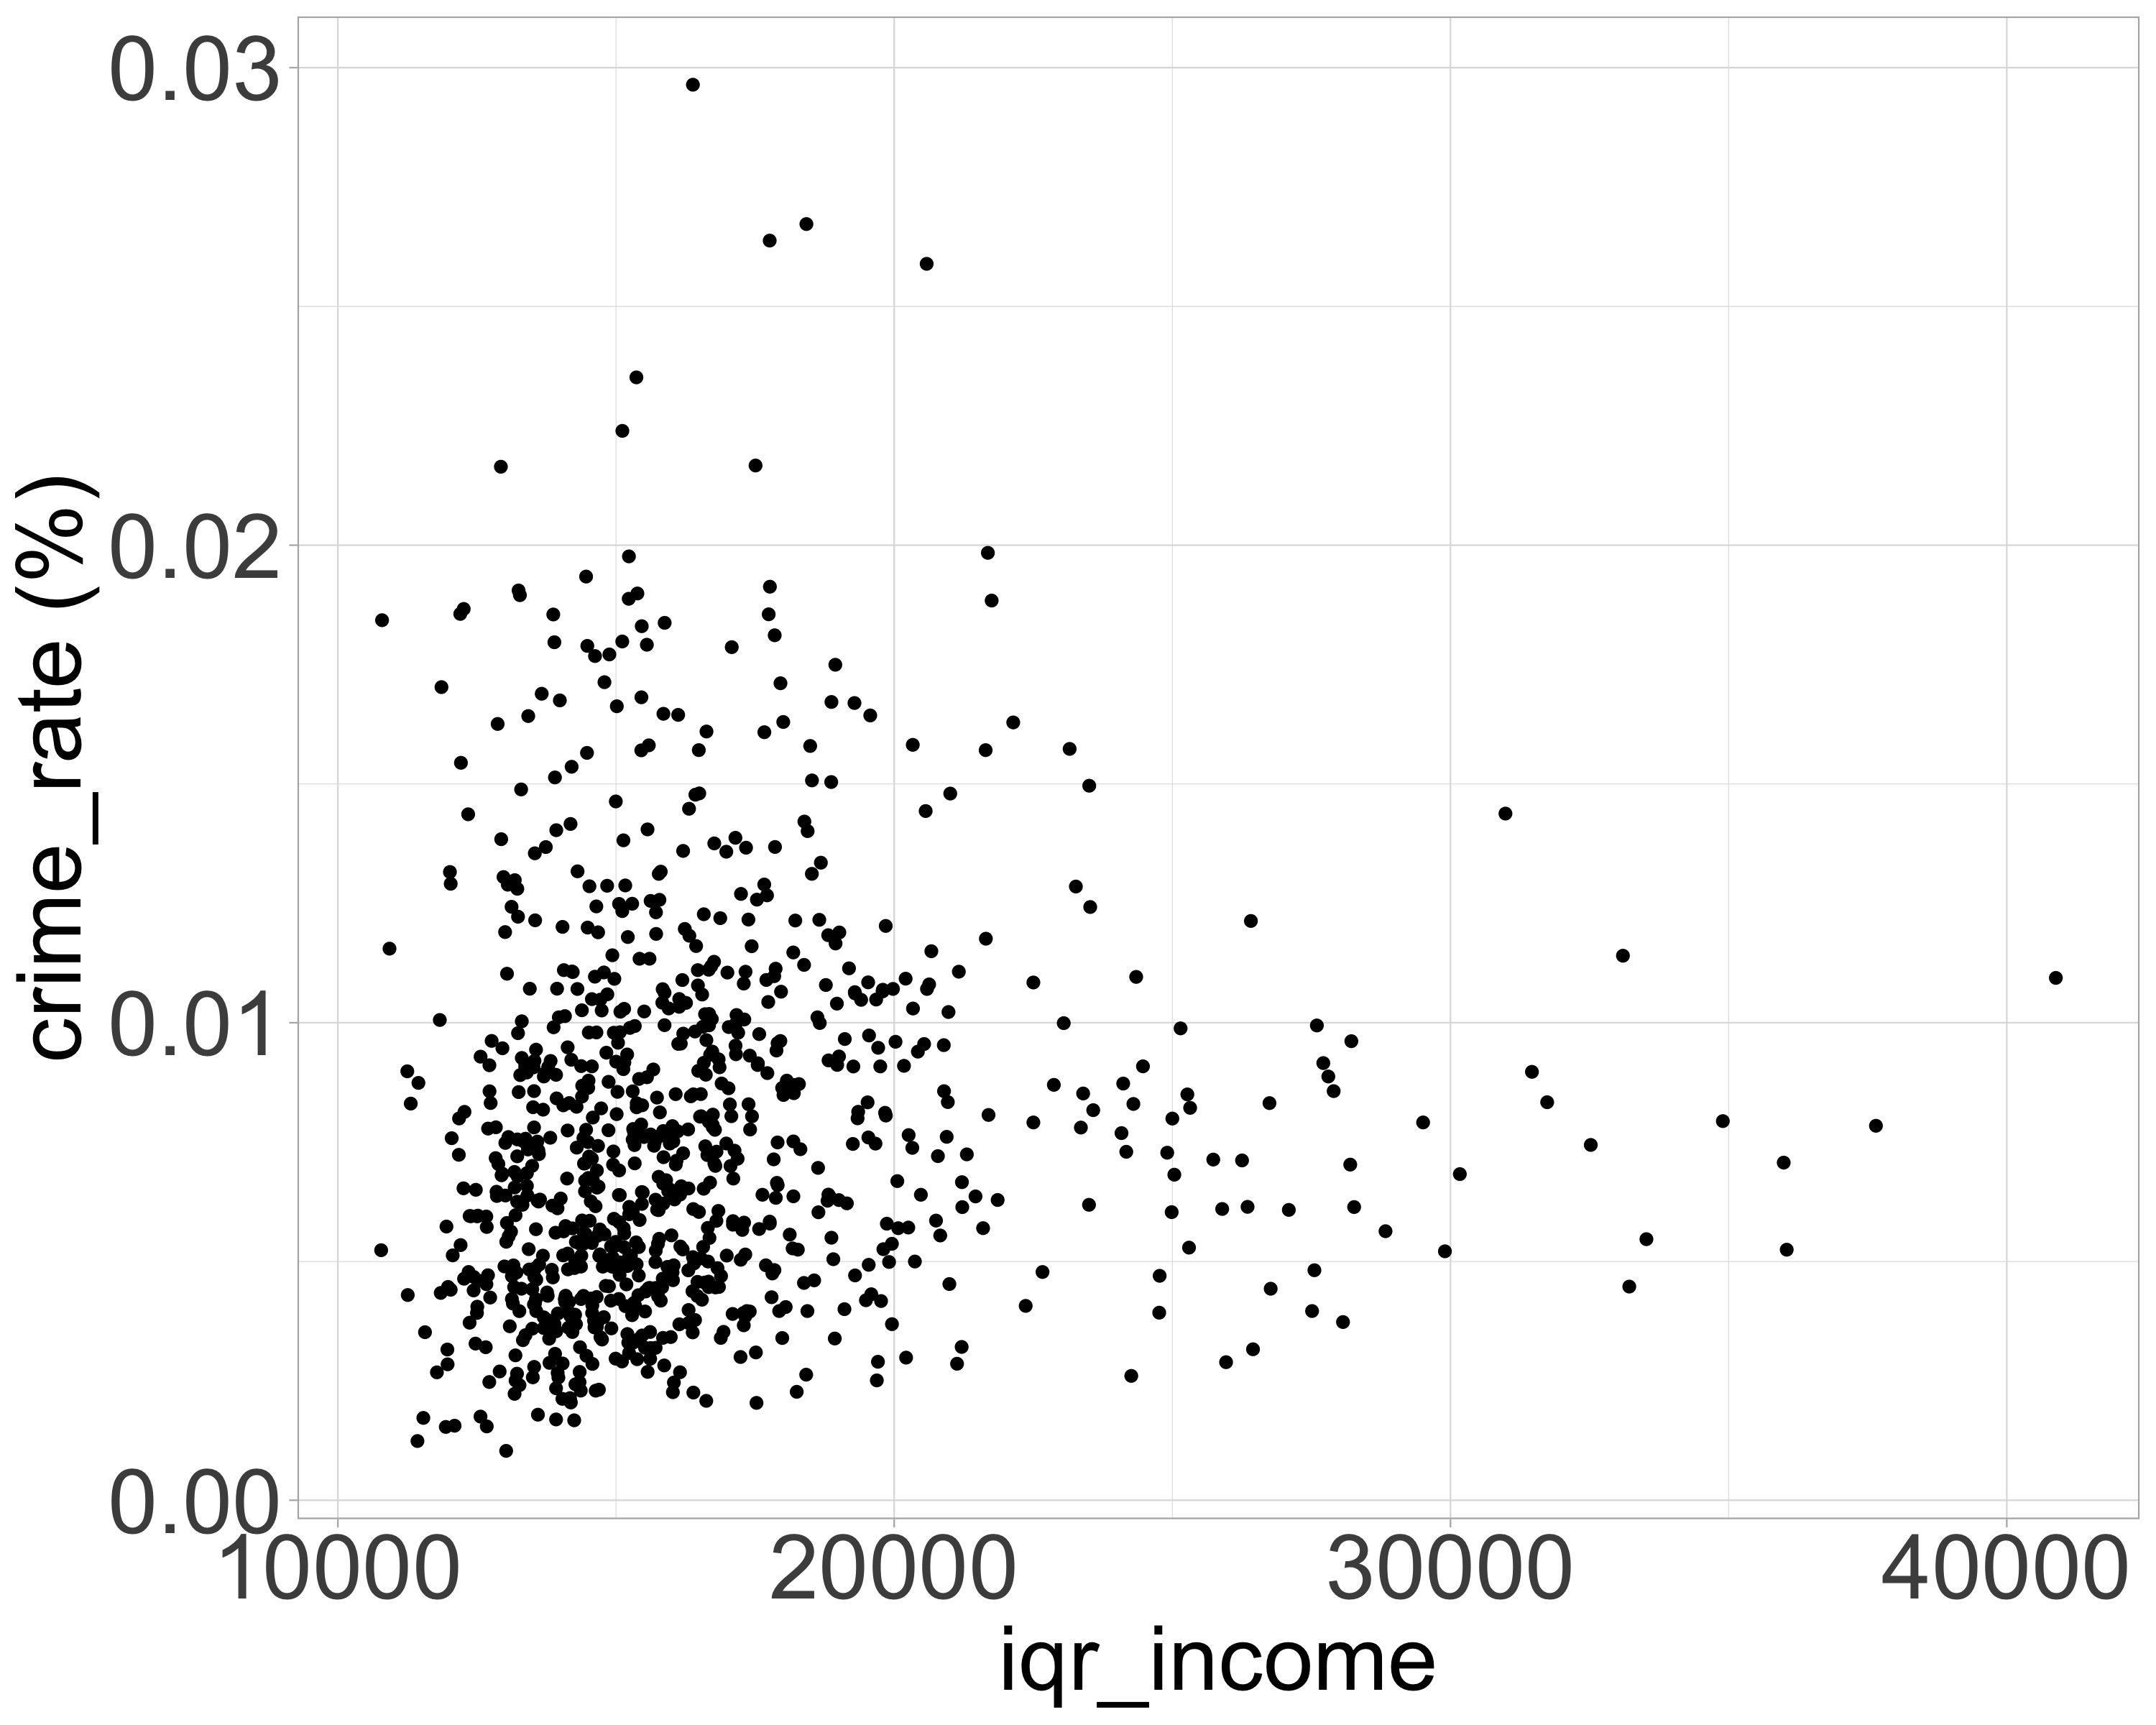
\includegraphics[width=\textwidth]{Exercise_3/OUTPUT/cr_iqr.png}
    \end{minipage}%
    \begin{minipage}{0.5\textwidth}
      \centering
      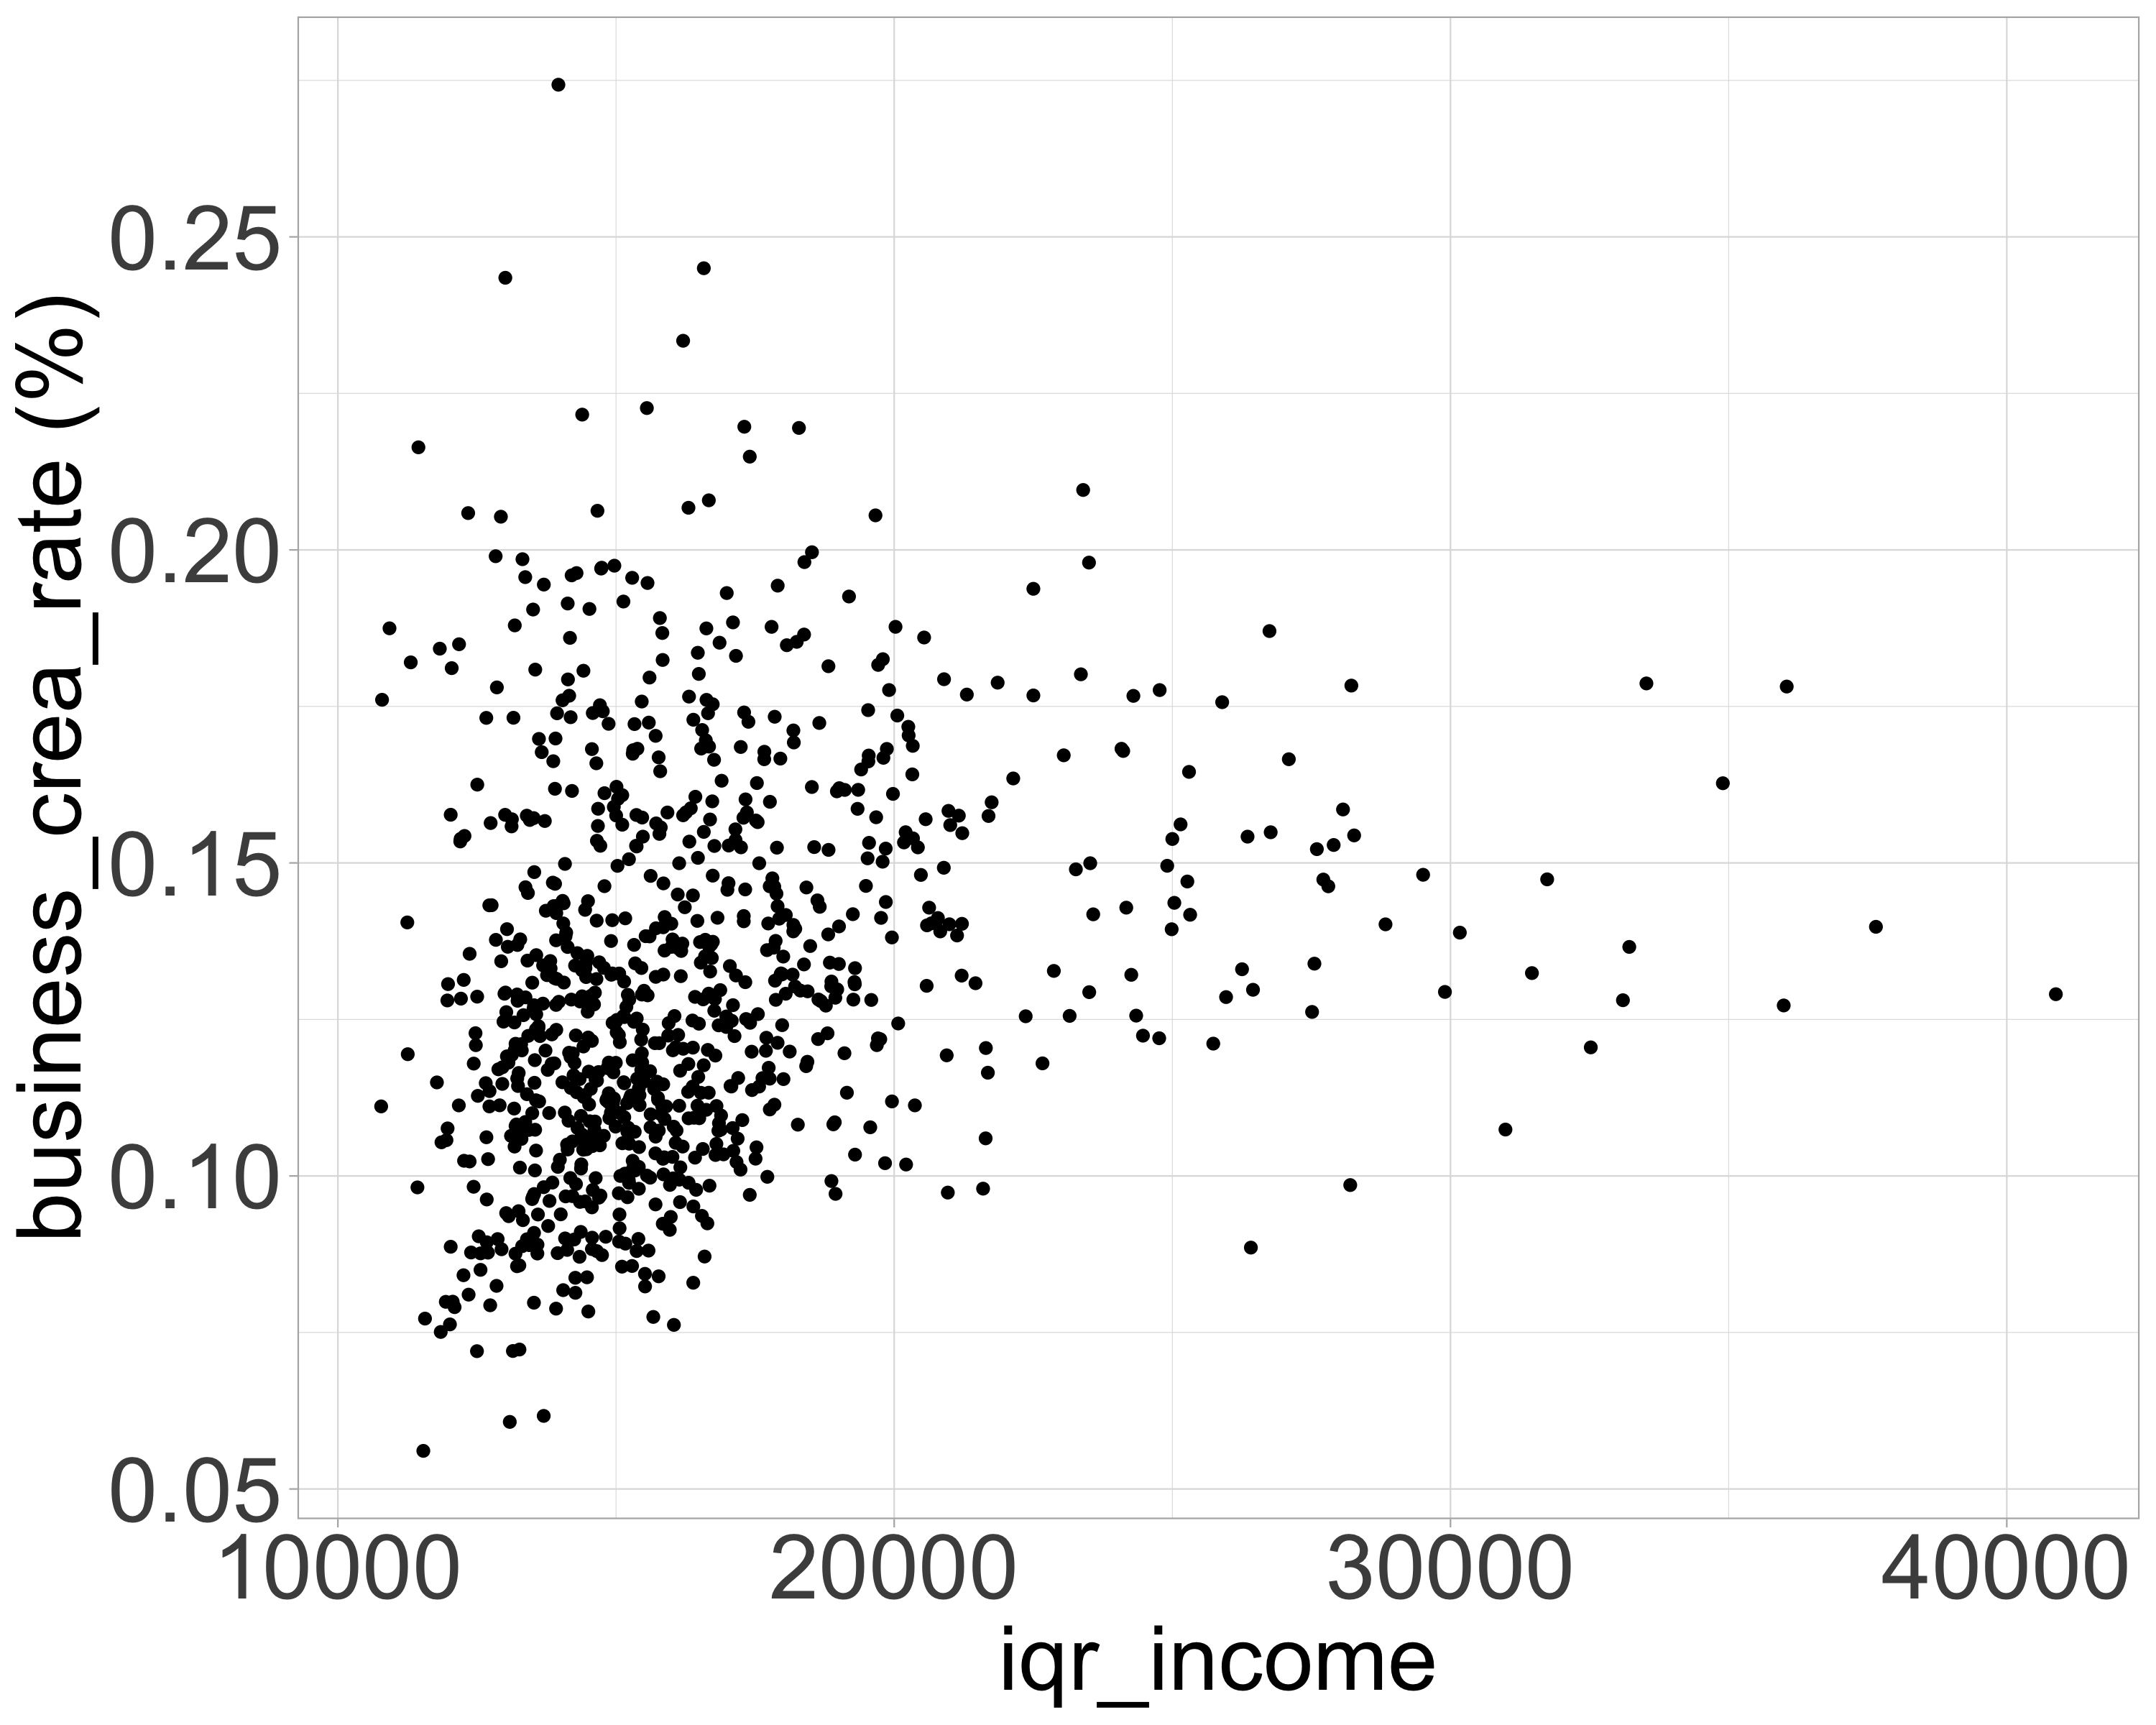
\includegraphics[width=\textwidth]{Exercise_3/OUTPUT/bcr_iqr.png}
    \end{minipage}
    \caption{Crime rate and business creation growth rate with respect to inequality indicator}
    \label{ineq}
  \end{figure}